
\begin{frame}{‌طولانی‌ترین زیر رشته مشترک}
\begin{itemize}\itemr
\item[-]
برخی مواقع زیست شناسان نیاز دارند دو یا چند ارگانیسم مختلف را با یکدیگر مقایسه کنند. برای این کار دی‌ان‌ای این ارگانیسم‌ها باید مقایسه شوند. یک رشتهٔ دی‌ان‌ای شامل رشته‌ای از مولکول‌ها به نام مولکول‌های پایه است که می‌توانند آدنین
\fn{1}{adenine}
، سیتوزین
\fn{2}{cytosine}
، گرانین
\fn{3}{granine}
، یا تیمین
\fn{4}{thymine}
باشند. هریک از این مولکول‌های پایه با یک حرف نشان داده می‌شوند، بنابراین یک رشته دی‌ان‌ای، یک رشته بر روی الفبای
\m{\{A, C, G, T \}}
است. برای مثال
\m{S_1 = ACCGGTC}
یک رشته دی‌ان‌ای است.
\item[-]
یکی از دلایلی که نیاز داریم دو رشتهٔ دی‌ان‌ای را با یکدیگر مقایسه کنیم، برای این است که متوجه شویم دو ارگانیسم چقدر به یکدیگر شباهت دارند.
\end{itemize}
\end{frame}


\begin{frame}{‌طولانی‌ترین زیر رشته مشترک}
\begin{itemize}\itemr
\item[-]
روش‌های مختلفی برای سنجش شباهت دو رشتهٔ دی‌ان‌ای وجود دارند.
%یک روش برای سنجش شباهت دو رشتهٔ دی‌ان‌ای این است که برای شباهت یک مقدار عددی تعریف کنیم. این مقدار عددی برابر است با تعداد تغییرات مورد نیاز در یک رشته برای به دست آوردن رشتهٔ دیگر.
\item[-]
یک روش برای سنجش شباهت این است که زیر رشته‌های مشترک بین دو رشته را پیدا کنیم. هرچقدر این زیر رشته‌های مشترک طول بیشتری داشته باشند، دو رشته به یکدیگر شبیه‌ترند.
\item[-]
در این روش برای مقایسه دو رشته باید زیر رشته‌های مشترک محاسبه شوند و طولانی‌ترین آنها پیدا شود. به این مسئله، مسئلهٔ پیدا کردن طولانی‌ترین زیر رشته مشترک
\fn{1}{longest common subsequence}
گفته می‌شود.
\end{itemize}
\end{frame}


\begin{frame}{‌طولانی‌ترین زیر رشته مشترک}
\begin{itemize}\itemr
\item[-]
یک زیر دنباله از یک دنباله، دنباله‌ای است که از حذف صفر یا بیشتر عنصر از دنباله اصلی به دست بیاید.
\item[-]
به طور رسمی، به ازای دنبالهٔ
\m{X = \langle x_1, x_2, \cdots , x_m \rangle}
، دنبالهٔ
\m{Z = \langle z_1, z_2, \cdots , z_k \rangle}
را زیر دنباله
\fn{1}{subsequence}
\m{X}
می‌نامیم اگر دنبالهٔ صعودی
\m{\langle i_1, i_2, \cdots , i_k \rangle}
از اندیس‌های
\m{X}
وجود داشته باشند، به طوری‌که به ازای
\m{j = 1,2, \cdots , k}
داشته باشیم
\m{x_{i_j} = z_j}.
\item[-]
 برای مثال دنبالهٔ
\m{Z = \langle B,C,D,B \rangle}
 یک زیردنباله از دنبالهٔ
\m{X = \langle A,B,C,B,D,A,B \rangle}
 است با اندیس‌های
\m{\langle 2,3,5,7 \rangle} .
\end{itemize}
\end{frame}


\begin{frame}{‌طولانی‌ترین زیر رشته مشترک}
\begin{itemize}\itemr
\item[-]
به ازای دو دنبالهٔ
\m{X}
و
\m{Y}
، می‌گوییم دنبالهٔ
\m{Z}
یک زیردنبالهٔ مشترک
\fn{1}{common subsequence}
\m{X}
و
\m{Y}
است اگر
\m{Z}
زیر دنباله‌ای از
\m{X}
و همچنین
\m{Y}
باشد.
\item[-]
برای مثال اگر
\m{X = \langle A,B,C,B,D,A,B \rangle}
و
\m{Y = \langle B,D,C,A,B,A \rangle}
باشند آنگاه
\m{\langle B,C,A \rangle}
یک زیردنبالهٔ مشترک
\m{X}
و
\m{Y}
است.
\item[-]
دنبالهٔ
\m{\langle B,C,A \rangle}
با طول ۳ طولانی‌ترین زیر دنبالهٔ مشترک
\m{X}
و
\m{Y}
نیست، چرا که دنبالهٔ
\m{\langle B,C,B,A \rangle}
با طول ۴ وجود دارد که زیر دنبالهٔ مشترک
\m{X}
و
\m{Y}
است. این زیردنباله، طولانی‌ترین زیر دنبالهٔ مشترک
\fn{2}{longest common subsequence}
\m{X}
و
\m{Y}
است، چرا که زیردنبالهٔ مشترک بلندتری وجود ندارد.
\end{itemize}
\end{frame}



\begin{frame}{‌طولانی‌ترین زیر رشته مشترک}
\begin{itemize}\itemr
\item[-]
می‌توانیم مسئله طولانی‌ترین زیردنبالهٔ مشترک را با استفاده از یک روش جستجوی کامل
\fn{1}{exhaustive search (brute-force search)}
به دست آوریم، بدین معنی که همهٔ زیردنباله‌های مشترک دو رشته را به دست آوریم و مقایسه کنیم. از آنجایی که رشته
\m{X}
با طول m تعداد
\m{2^m}
زیردنباله دارد، بنابراین این روش برای رشته‌های طولانی غیر قابل استفاده است.
\item[-]
می‌خواهیم این مسئله را به روش برنامه‌ریزی پویا حل کنیم.
\end{itemize}
\end{frame}



\begin{frame}{‌طولانی‌ترین زیر رشته مشترک}
\begin{itemize}\itemr
\item[-]
گام اول : مشخص کردن ساختار جواب مسئله بر اساس زیرمسئله‌ها
\item[-]
برای تعریف مسئله طولانی‌ترین زیررشتهٔ مشترک با استفاده از زیر مسئله‌ها، ابتدا مفهوم پیشوند
\fn{1}{prefix}
یک دنباله را تعریف می‌کنیم.
\item[-]
به ازای دنبالهٔ
\m{X = \langle x_1, x_2, \cdots , x_m \rangle}،
i
امین پیشوند
\m{X}
برابراست با
\m{X_i = \langle x_1, x_2, \cdots , x_i \rangle}
به ازای
\m{i = 0,1, \cdots , m}.
\item[-]
برای مثال اگر
\m{X = \langle A,B,C,B,D,A,B \rangle}
باشد، آنگاه
\m{X_4 = \langle A,B,C,B \rangle}
و
\m{X_0}
دنبالهٔ تهی است.
\end{itemize}
\end{frame}


\begin{frame}{‌طولانی‌ترین زیر رشته مشترک}
\begin{itemize}\itemr
\item[-]
فرض کنید
\m{X = \langle x_1, x_2, \cdots , x_m \rangle}
و
\m{Y = \langle y_1, y_2, \cdots , y_n \rangle}
دو دنباله باشند و
\m{Z = \langle z_1, z_2, \cdots , z_k \rangle}
طولانی‌ترین زیررشته مشترک
\m{X}
و
\m{Y}
باشد. خواهیم داشت :
\item[۱-]
اگر
\m{x_m = y_n}
آنگاه
\m{z_k = x_m = y_n}
و
\m{Z_{k-1}}
طولانی‌ترین زیر رشته مشترک
\m{X_{m-1}}
و
\m{Y_{n-1}}
است.
\item[۲-]
اگر
\m{x_m \neq y_n}
و
\m{z_k \neq x_m}
باشد، آنگاه
\m{Z}
طولانی‌ترین زیر رشته مشترک
\m{X_{m-1}}
و
\m{Y}
است.
\item[۳-]
اگر
\m{x_m \neq y_n}
و
\m{z_k \neq y_n}
باشد، آنگاه
\m{Z}
طولانی‌ترین زیر رشته مشترک
\m{X}
و
\m{Y_{n-1}}
است.
\end{itemize}
\end{frame}


\begin{frame}{‌طولانی‌ترین زیر رشته مشترک}
\begin{itemize}\itemr
\item[-]
گزاره‌های ۱، ۲ ، ۳ در قضیه قبل را به ترتیب اثبات می‌کنیم.
\item[۱-]
اگر
\m{x_m = y_n}
آنگاه
\m{z_k = x_m = y_n}
و
\m{Z_{k-1}}
طولانی‌ترین زیر رشته مشترک
\m{X_{m-1}}
و
\m{Y_{n-1}}
است.
\\~
\\~
اثبات: اگر
\m{x_m = y_n}
باشد، الزاما باید داشته باشیم
\m{z_k = x_m}.
این گزاره را با برهان خلف ثابت می‌کنیم. فرض کنید
\m{z_k \neq x_m}
، آنگاه می توانیم
\m{x_m}
که برابر با
\m{y_n}
است را به
\m{Z}
بیافزاییم و زیررشته مشترکی پیدا کنیم که طول آن
\m{k+1}
است. از آنجایی که در صورت مسئله گفته شده
\m{Z}
طولانی‌ترین زیر رشته مشترک با طول
\m{k}
است، پس به تناقض می‌رسیم. پس فرض اولیه نادرست است و الزاما باید داشته باشیم
\m{z_k = x_m = y_n}.
\iffalse
پس
\m{Z_{k-1}}
یعنی
\m{k-1}
امین پیشوند
\m{Z}
باید یک زیررشته مشترک
\m{X_{m-1}}
و
\m{Y_{n-1}}
باشد.
\fi
حال باید ثابت کنیم
\m{Z_{k-1}}
طولانی‌ترین زیر رشته مشترک
\m{X_{m-1}}
و
\m{Y_{n-1}}
نیز هست. این گزاره را با برهان خلف ثابت می‌کنیم. فرض یک زیر رشته مشترک
\m{W}
برای
\m{X_{m-1}}
و
\m{Y_{n-1}}
وجود دارد که طول آن از
\m{k-1}
بیشتر است. در اینصورت با اضافه کردن
\m{x_m = y_n}
به
\m{W}
زیر رشته‌ای ساخته می‌شود که طول آن از
\m{k}
بیشتر است. اما در اینجا به تناقض می‌رسیم چون فرض کردیم طول بلندترین زیر رشته مشترک
\m{k}
است.
\end{itemize}
\end{frame}


\begin{frame}{‌طولانی‌ترین زیر رشته مشترک}
\begin{itemize}\itemr
\item[۲-]
اگر
\m{x_m \neq y_n}
و
\m{z_k \neq x_m}
باشد، آنگاه
\m{Z}
طولانی‌ترین زیر رشته مشترک
\m{X_{m-1}}
و
\m{Y}
است.
\\~
\\~
اثبات: اگر
\m{z_k \neq x_m}
باشد، آنگاه
\m{Z}
یک زیر رشته مشترک برای
\m{X_{m-1}}
و
\m{Y}
است. اگر یک زیر رشته مشترک دیگر به نام
\m{W}
با طول بیشتر از
\m{k}
برای
\m{X_{m-1}}
و
\m{Y}
وجود داشت، آنگاه
\m{W}
می‌توانست یک زیر رشته مشترک برای
\m{X}
و
\m{Y}
نیز باشد که این متناقض است با فرض اینکه
\m{Z}
بلندترین زیر رشته مشترک
\m{X}
و
\m{Y}
با طول
\m{k}
است.
\item[۳-]
اگر
\m{x_m \neq y_n}
و
\m{z_k \neq y_n}
باشد، آنگاه
\m{Z}
طولانی‌ترین زیر رشته مشترک
\m{X}
و
\m{Y_{n-1}}
است.
\\~
\\~
اثبات: شبیه و متقارن حالت ۲ است.
\end{itemize}
\end{frame}


\begin{frame}{‌طولانی‌ترین زیر رشته مشترک}
\begin{itemize}\itemr
\item[-]
بنابراین توانستیم مسئله طولانی‌ترین زیر رشته مشترک را بر اساس زیر مسئله‌های بهینه آن تعریف کنیم. جواب زیر مسئله‌های در همهٔ حالت‌های بررسی شده در جواب مسئله وجود دارد.
\item[-]
پس این مسئله دارای زیرساختار بهینه است.
\end{itemize}
\end{frame}



\begin{frame}{‌طولانی‌ترین زیر رشته مشترک}
\begin{itemize}\itemr
\item[-]
گام دوم : تعریف کردن مقدار جواب به صورت بازگشتی
\item[-]
فرض کنید 
\m{c[i,j]}
طول بلندترین زیررشتهٔ مشترک 
\m{X_i}
و
\m{Y_j}
باشد.
\item[-]
 این مسئله بهینه‌سازی را می‌توانیم بر اساس زیر ساختارهای بهینه به صورت زیر تعریف کنیم.
\begin{align*}
\m{c[i,j]} = \left\{\begin{array}{lr}
          \m{0}& \m{j = 0}~\text{یا}~\m{i = 0}~\text{اگر}\\
          \m{c[i-1,j-1] + 1}& \m{x_i = y_j}~\text{و}~\m{i,j > 0}~\text{اگر}\\
          \m{\max \{c[i,j-1],c[i-1,j] \}}& \m{x_i \neq y_j}~\text{و}~\m{i,j > 0}~\text{اگر}
\end{array}\right.
\end{align*}
\item[-]
دقت کنید که اگر الگوریتم بازگشتی برای حل این مسئله استفاده شود زیر مسئله‌ها به طور تکراری محاسبه می‌شوند. پس می‌توانیم در این‌جا از برنامه‌ریزی پویا استفاده کنیم.
\end{itemize}
\end{frame}



\begin{frame}{‌طولانی‌ترین زیر رشته مشترک}
\begin{itemize}\itemr
\item[-]
گام سوم : محاسبه طول طولانی‌ترین زیر دنباله مشترک
\item[-]
از آنجایی که برای دو دنباله
\m{X = \langle x_1, x_2, \cdots , x_m \rangle}
و
\m{Y = \langle y_1, y_2, \cdots , y_n \rangle}
مقادیر جدول
\m{c[0:m,0:n]}
باید محاسبه شوند و هر خانه از جدول در زمان ثابت
\ath{1}
محاسبه می‌شود، بنابراین زمان اجرای الگوریتم برنامه‌ریزی پویا برای این مسئله برابراست با
\ath{mn}
. طول زیر رشته مشترک برابراست با مقدار محاسبه شده برای
\m{c[m,n]}.
\end{itemize}
\end{frame}


\begin{frame}{‌طولانی‌ترین زیر رشته مشترک}
\begin{itemize}\itemr
\item[-]
الگوریتم طولانی‌ترین زیررشته مشترک به صورت زیر نوشته شده است.
\begin{algorithm}[H]\alglr
  \caption{Longest Common Subsequence Length} 
  \begin{algorithmic}[1]
   \Func{LCS-Length}{X,Y, m, n} 
    \State let b[1:m, 1:n] and c[0:m, 0:n] be new tables
    	\For{i = 1 \To m} 
      		\State c[i,0] = 0
       \EndFor
    	\For{j = 0 \To n} 
      		\State c[0,j] = 0
       \EndFor                                       
  \end{algorithmic}
  \label{alg:merge}
\end{algorithm}
\end{itemize}
\end{frame}


\begin{frame}{‌طولانی‌ترین زیر رشته مشترک}
\begin{itemize}\itemr
\item[-]
\begin{algorithm}[H]\alglr
  \caption{Longest Common Subsequence Length} 
  \begin{algorithmic}[1]
   \setcounter{ALG@line}{5}
   \Func{LCS-Length}{X,Y, m, n} 
    	\For{i = 1 \To m} \LeftComment{compute table entries in row-major order} 
        	\For{j = 1 \To n}
        		\If{X[i] == Y[j]}
        			\State c[i, j] = c[i-1, j-1] + 1
        			\State b[i, j] = "$\nwarrow$"
        		\ElsIf{c[i-1, j] $\geqslant$ c[i, j-1]}
        			\State c[i, j] = c[i-1, j] 
        			\State b[i, j] = "$\uparrow$"
        		\Else
        		    \State c[i, j] = c[i, j-1]
        			\State b[i, j] = "$\leftarrow$"
        		\EndIf
        	\EndFor
        \EndFor
    \State \Return c and b	                                         
  \end{algorithmic}
  \label{alg:merge}
\end{algorithm}
\end{itemize}
\end{frame}


\begin{frame}{‌طولانی‌ترین زیر رشته مشترک}
\begin{itemize}\itemr
\item[-]
گام چهارم : ساختن بلندترین زیر دنبالهٔ مشترک
\item[-]
با استفاده از جدول b که توسط الگوریتم قبل ساخته شده می‌توانیم زیر دنبالهٔ مشترک
\m{X}
و
\m{Y}
را بسازیم، بدین ترتیب که با
\m{b[m,n]}
شروع می‌کنیم و جهت نشانه‌ها را دنبال می‌کنیم. علامت
\m{\nwarrow}
در جدول b نشان می‌دهد که
\m{x_i = y_j}
در طولانی‌ترین زیررشتهٔ مشترک است.
\end{itemize}
\end{frame}


\begin{frame}{‌طولانی‌ترین زیر رشته مشترک}
\begin{itemize}\itemr
\item[-]
برای مثال به ازای دو دنبالهٔ
\m{X = \langle A,B,C,B,D,A,B \rangle}
و
\m{Y = \langle B,D,C,A,B,A \rangle}
جدول زیر به‌دست می‌آید.
\begin{figure}
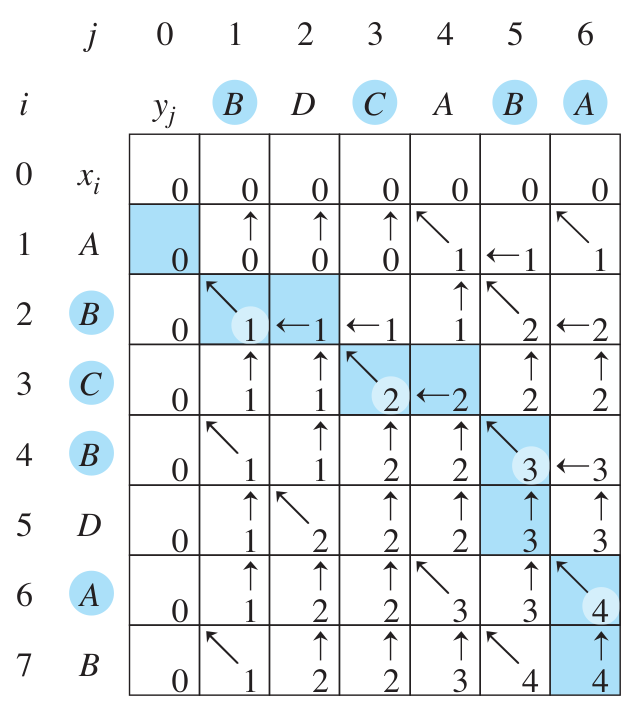
\includegraphics[width=0.4\textwidth]{figs/chap04/lcs-example}
\end{figure}
\end{itemize}
\end{frame}


\begin{frame}{‌طولانی‌ترین زیر رشته مشترک}
\begin{itemize}\itemr
\item[-]
\begin{algorithm}[H]\alglr
  \caption{Print Longest Common Subsequence} 
  \begin{algorithmic}[1]
   \Func{Print-LCS}{b, X, i, j}
		\If{i == 0 or j ==0}
				\State \Return \LeftComment{the longest common subsequence has length 0}
		\EndIf
		\If{b[i, j] == "$\nwarrow$"}
			\State Print-LCS(b, X, i-1, j-1)
			\State print X[i] \LeftComment{same as Y[j]}
		\ElsIf{b[i, j] = "$\uparrow$"}
			\State Print-LCS(b, X, i-1, j)
		\Else{\State Print-LCS(b, X, i, j-1)}
		\EndIf
  \end{algorithmic}
  \label{alg:merge}
\end{algorithm}  
\end{itemize}
\end{frame}




\begin{frame}{‌طولانی‌ترین زیر رشته مشترک}
\begin{itemize}\itemr
\item[-]
پس از طراحی یک الگوریتم معمولاً به دنبال روش‌هایی برای بهبود در زمان اجرا و میزان حافظه می‌گردیم.
\item[-]
در الگوریتم طولانی‌ترین زیر دنبالهٔ مشترک به طور مثال می توانیم جدول b را حذف کنیم و اطلاعات لازم برای ساختن بلندترین زیر دنبالهٔ مشترک را از جدول c به دست آوریم.
\item[-]
هریک از درایه‌های
\m{c[i,j]}
از طریق یکی از سه درایهٔ
\m{c[i-1,j-1]}
،
\m{c[i-1,j]}
،
\m{c[i,j-1]}
محاسبه شده است که در زمان ثابت می‌توانیم بدون جدول b به دست آوریم درایه
\m{c[i,j]}
چگونه محاسبه شده است.
\item[-]
بنابراین طولانی‌ترین زیردنبالهٔ مشترک را می‌توانیم همچنان در زمان
\ath{m+n}
بسازیم و جدول b را حذف کرده و از حافظهٔ مورد نیاز به میزان
mn
بکاهیم.
\end{itemize}
\end{frame}
